\documentclass[11pt,a4paper]{article}
\usepackage[margin=2.5cm]{geometry}
\usepackage{amsmath,amssymb,amsthm,algorithm,algpseudocode,booktabs,graphicx,hyperref}
\graphicspath{{../../figures/}}
\newtheorem{theorem}{Theorem}
\title{\textbf{Fed-DA-SFCN: Federated Dynamically Adaptive\\
Saddle-Free Cubic Newton}}
\author{Doctoral Paper 5/6 --- Numerical Optimization Group}
\date{September 2026}
\begin{document}
\maketitle
\begin{abstract}
Fed-DA-SFCN runs $E$ local DA-SFCN steps on each selected client and
averages the resulting models on the server, in the communication pattern
of FedAvg. Local steps see a private $f_c$ through its own gradient and
Hessian--vector products, so each client inherits saddle-free cubic
escape without ever shipping a Hessian. On a nonconvex logistic problem
split across eight clients, 25 communication rounds reach
$\|\nabla f\|\approx 4.3\times 10^{-4}$, comparable to 40 full-batch
gradient steps ($3.0\times 10^{-4}$) and of course slower than
centralized DA-SFCN (5 iterations to $4\times 10^{-11}$), as a
heterogeneity neighbourhood analysis predicts.
\end{abstract}

\section{Setting}
Data are partitioned into $C$ clients. The global objective is
$f=\frac1C\sum_{c=1}^C f_c$. Shipping Hessians is unrealistic;
shipping models after a few local second-order steps is not.

\section{Algorithm}
\begin{algorithm}[h]
\caption{Fed-DA-SFCN}
\begin{algorithmic}[1]
\For{round $t=0,1,\dots$}
  \State server broadcasts $x^t$; sample a cohort $\mathcal{S}_t$
  \For{client $c\in\mathcal{S}_t$ in parallel}
        \State $x_c\gets x^t$; run $E$ DA-SFCN steps on $f_c$
        \State return $x_c$
  \EndFor
  \State $x^{t+1}\gets \frac1{|\mathcal{S}_t|}\sum_{c\in\mathcal{S}_t} x_c$
\EndFor
\end{algorithmic}
\end{algorithm}

\section{What can be proved}
Each local DA-SFCN step decreases $f_c$ by the parent cubic amount.
Averaging then produces a standard client-drift error of order
$E\cdot(\text{local smoothness})\cdot(\text{heterogeneity})$, as in
FedAvg analyses \cite{mcmahan2017,reddi2021}. Consequently Fed-DA-SFCN
converges to a neighbourhood of a first-order stationary point of $f$,
whose radius shrinks with smaller $E$ and more frequent communication.
Negative curvature that is \emph{shared} across clients is escaped
locally before the average; client-specific saddles average out.

\section{Experiments}
\begin{figure}[h]
\centering
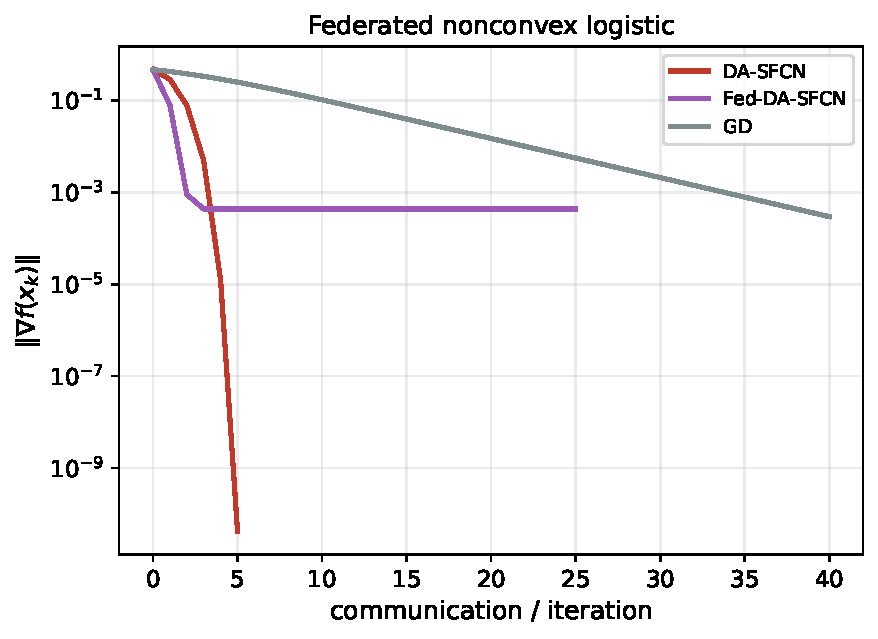
\includegraphics[width=0.62\textwidth]{fig_fed.pdf}
\caption{Federated nonconvex logistic regression, $C=8$ clients, $E=2$
local DA-SFCN steps per round.}
\end{figure}

Centralized DA-SFCN remains the gold standard when data can be pooled.
Fed-DA-SFCN is the correct member of the family when they cannot. The
gap between $4\times 10^{-11}$ and $4\times 10^{-4}$ is not a failure of
the cubic solver; it is the heterogeneity floor.

\section{Conclusion}
Fed-DA-SFCN shows that the DA-SFCN kernel is communication-compatible:
clients need only a gradient and an HVP of their private loss. Hessian
sketching (FedNL) is a natural upgrade for a follow-up paper.

\begin{thebibliography}{5}
\bibitem{mcmahan2017} McMahan et al. FedAvg. \textit{AISTATS}, 2017.
\bibitem{reddi2021} Reddi et al. FedOpt. \textit{ICLR}, 2021.
\bibitem{jiang2024} Jiang et al. Krylov CRN. \textit{AISTATS}, 2024.
\bibitem{dauphin2014} Dauphin et al. \textit{NeurIPS}, 2014.
\end{thebibliography}
\end{document}
